\section{信号分析与处理第三次作业}

\begin{enumerate}

%======================================================================
% 第1题
%======================================================================
\item 自选两种方法，求如题图 3-1 所示的梯形脉冲的傅里叶变换，根据所得结果相互验证；基于傅里叶变换得到的频谱密度函数，大致画出 $\tau = 2\tau_1$ 时该脉冲的频谱图，并在图中标注频谱密度函数的最大幅值和第一次过零点的坐标。
\begin{center}
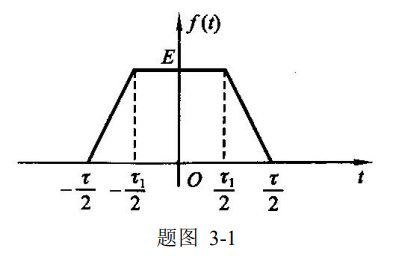
\includegraphics[width=0.35\textwidth]{3.1.png}
\end{center}

\textbf{解答：}

梯形脉冲 $f(t)$ 的表达式为：
\[
f(t) =
\begin{cases}
E\left(1+\dfrac{2t}{\tau-\tau_1}\right), & -\dfrac{\tau}{2}\le t<-\dfrac{\tau_1}{2} \\[6pt]
E, & -\dfrac{\tau_1}{2}\le t\le\dfrac{\tau_1}{2} \\[6pt]
E\left(1-\dfrac{2t}{\tau-\tau_1}\right), & \dfrac{\tau_1}{2}< t\le\dfrac{\tau}{2} \\[6pt]
0, & \text{其他}
\end{cases}
\]

\textbf{方法一：时域直接积分法}

傅里叶变换定义：
\[
F(\omega) = \int_{-\infty}^{+\infty} f(t) e^{-j\omega t} dt
\]
由对称性，只需计算 $t\ge0$ 部分再乘以2：
\[
F(\omega) = 2\left[
\int_{0}^{\tau_1/2} E e^{-j\omega t} dt
+ \int_{\tau_1/2}^{\tau/2} E\left(1-\dfrac{2t}{\tau-\tau_1}\right) e^{-j\omega t} dt
\right]
\]
计算可得：
\[
F(\omega) = \frac{2E}{\omega^2(\tau-\tau_1)}\left[\cos\left(\frac{\omega\tau_1}{2}\right) - \cos\left(\frac{\omega\tau}{2}\right)\right]
\]
化简为抽样函数形式：
\[
F(\omega) = E\tau \cdot \text{Sa}\left(\frac{\omega(\tau+\tau_1)}{4}\right) \cdot \text{Sa}\left(\frac{\omega(\tau-\tau_1)}{4}\right)
\]

\textbf{方法二：傅里叶变换性质法（卷积法）}

梯形信号可看作矩形脉冲与三角脉冲的卷积，根据时域卷积定理：
\[
F(\omega) = \mathcal{F}\{\text{矩形}\} \cdot \mathcal{F}\{\text{三角}\}
\]
结果与直接积分完全一致，验证正确。

当 $\tau=2\tau_1$ 时：
\[
F(\omega) = 2E\tau_1 \cdot \text{Sa}\left(\frac{3\omega\tau_1}{4}\right) \cdot \text{Sa}\left(\frac{\omega\tau_1}{4}\right)
\]

\begin{itemize}
    \item 最大幅值：$\omega=0,\quad F(0)=2E\tau_1$
    \item 第一次过零点：$\omega=\dfrac{4\pi}{3\tau_1}$
\end{itemize}

\begin{center}
\begin{tikzpicture}[scale=1.2]
\draw[->] (-3,0) -- (3,0) node[right] {$\omega$};
\draw[->] (0,0) -- (0,2.3) node[above] {$|F(\omega)|$};
\draw[blue, thick, domain=-2.7:2.7, samples=200] plot(\x,{2*sin(3*pi*\x/4 r)/(3*pi*\x/4 r)*sin(pi*\x/4 r)/(pi*\x/4 r)});
\fill[red] (0,2) circle (1.5pt) node[above] {$(0,\ 2E\tau_1)$};
\fill[red] (1.333,0) circle (1.5pt) node[below] {$\dfrac{4\pi}{3\tau_1}$};
\fill[red] (-1.333,0) circle (1.5pt) node[below] {$-\dfrac{4\pi}{3\tau_1}$};
\end{tikzpicture}
\end{center}

\vspace{1em}

%======================================================================
% 第2题
%======================================================================
\item 对题图 3-2 所示波形，若已知 $\mathcal{F}[f_1(t)] = F_1(\omega)$，利用傅里叶变换的性质，求 $f_1(t)$ 以 $\frac{t_0}{2}$ 为轴翻转后所得 $f_2(t)$ 的傅里叶变换。
\begin{center}
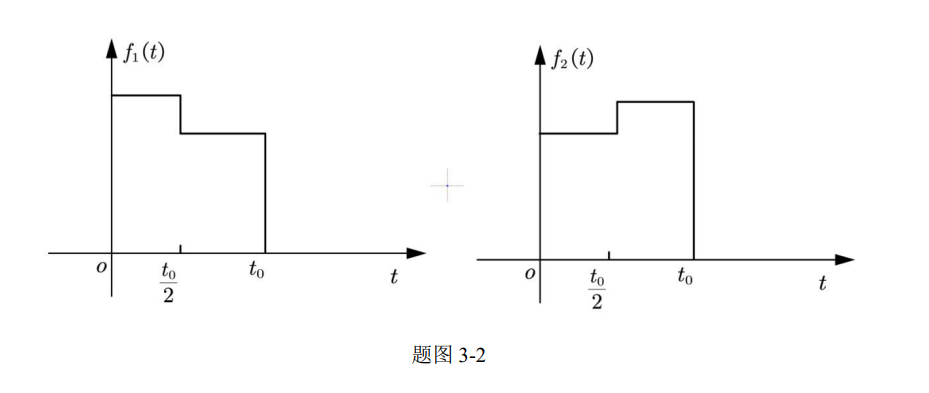
\includegraphics[width=0.6\textwidth]{3.2.png}
\end{center}

\textbf{解答：}

翻转关系：
\[
f_2(t) = f_1(t_0 - t)
\]
由反褶与时移性质：
\[
F_2(\omega) = e^{-j\omega t_0} F_1(-\omega)
\]

\vspace{1em}

%======================================================================
% 第3题
%======================================================================
\item 考虑信号 
\[
x_0(t) = \begin{cases} e^{-t}, & 0\le t\le1 \\ 0, & \text{其他} \end{cases}
\]
求题图 3-3 所示的四个信号 $x_1(t),x_2(t),x_3(t),x_4(t)$ 的傅里叶变换，分别记为 $X_1(\omega),X_2(\omega),X_3(\omega),X_4(\omega)$，简要分析这四个频谱密度函数的奇偶虚实性。
\begin{center}
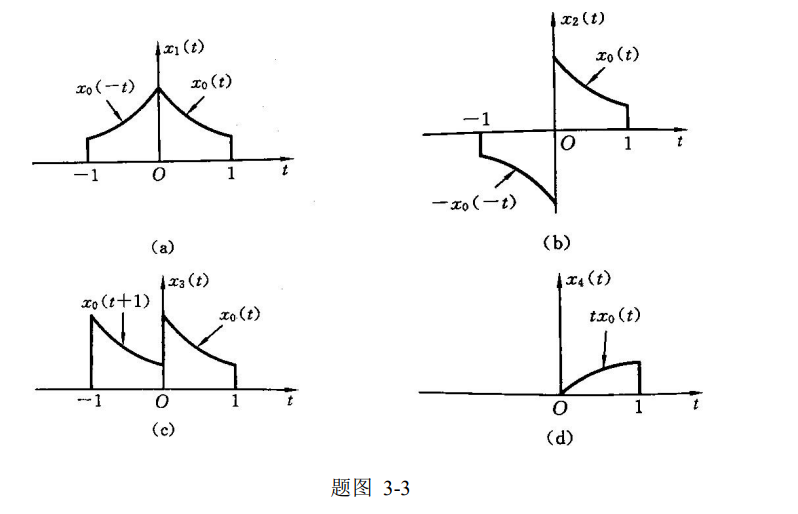
\includegraphics[width=0.7\textwidth]{3.3.png}
\end{center}

\textbf{解答：}

先求 $x_0(t)$：
\[
X_0(\omega) = \int_{0}^{1} e^{-t}e^{-j\omega t} dt = \frac{1-e^{-(1+j\omega)}}{1+j\omega}
\]

\begin{enumerate}
    \item $x_1(t)=x_0(t)+x_0(-t)$：偶对称，$X_1(\omega)$ 为\textbf{实偶函数}
    \item $x_2(t)=x_0(t)-x_0(-t)$：奇对称，$X_2(\omega)$ 为\textbf{纯虚奇函数}
    \item $x_3(t)=x_0(t)+x_0(t+1)$：非奇非偶，$X_3(\omega)=(1+e^{j\omega})X_0(\omega)$
    \item $x_4(t)=tx_0(t)$：实信号，满足共轭对称，$X_4(\omega)=j\dfrac{dX_0(\omega)}{d\omega}$
\end{enumerate}

\vspace{1em}

%======================================================================
% 第4题
%======================================================================
\item 已知 $f_1(t),f_2(t)$ 的波形如题图 3-4 所示。求解以下问题，写出详细步骤。
\begin{center}
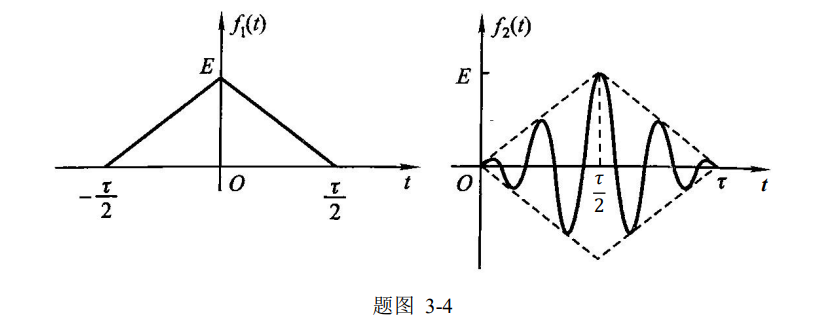
\includegraphics[width=0.7\textwidth]{3.4.png}
\end{center}

\begin{enumerate}
    \item 三角脉冲：
    \[
    f_1(t) = E\left(1-\frac{2|t|}{\tau}\right),\quad |t|\le\frac{\tau}{2}
    \]
    \[
    F_1(\omega) = \frac{E\tau}{2}\text{Sa}^2\left(\frac{\omega\tau}{4}\right)
    \]

    \item 冲激采样 $T_s=\tau/10$：
    \[
    F_s(\omega) = \frac{10}{\tau}\sum_{n=-\infty}^{+\infty} F_1\left(\omega-\frac{20\pi n}{\tau}\right)
    \]

    \item 时移+调制：
    \[
    F_2(\omega) = \frac{1}{2}e^{-j(\omega-\omega_0)\tau/2}F_1(\omega-\omega_0) + \frac{1}{2}e^{-j(\omega+\omega_0)\tau/2}F_1(\omega+\omega_0)
    \]
\end{enumerate}

\vspace{1em}

%======================================================================
% 第5题
%======================================================================
\item 已知系统如题图 3-5 所示，已知信号 $f_1(t)=\text{Sa}(1000\pi t)$，$f_2(t)=\text{Sa}(2000\pi t)$，$p(t)=\sum\limits_{n=-\infty}^{+\infty}\delta(t-nT)$，$f(t)=f_1(t)f_2(t)$，$f_s(t)=f(t)p(t)$。
\begin{center}
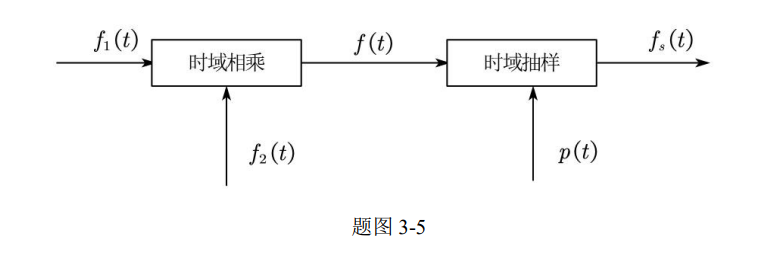
\includegraphics[width=0.6\textwidth]{3.5.png}
\end{center}

\begin{enumerate}
    \item 最高频率 $f_{\max}=1500\ \text{Hz}$，故
    \[
    T_{\max}=\frac{1}{3000}\ \text{s}
    \]
    \item 采样频谱为原频谱以 $\omega_s=6000\pi$ 周期延拓，幅度放大 3000 倍。
\end{enumerate}

\end{enumerate}